\chapter{Anexo} \label{chp:anexo}

\section{Conceptos Básicos}

\subsection{Hidrostática} \label{chp:anexo:hidrostatica}

Para representar las propiedades de un fluido en reposo, como la presión, en función de la altura y la densidad, se utiliza comúnmente la ecuación de la hidrostática, que es una aproximación matemática que se aplica a fluidos en condiciones normales de temperatura y presión.

La ecuación de la hidrostática establece que la presión, la altura, la densidad y la aceleración gravitacional del fluido están relacionados \cite{libro_fisica_giancoli}, mediante la siguiente fórmula:

\begin{equation}
    \label{eq:hidrostatica}
    P=\rho gh 
\end{equation}

Donde en ecuación \ref{eq:hidrostatica}:

\begin{itemize}
    \item $P$ es la presión del fluido (en Pascales)
    \item $\rho$ es la densidad del fluido en $kg/m^{3}$   
    \item $g$ es la aceleración gravitacional (en $m/s^{2}$
    \item $h$ es la altura del fluido (en metros)
\end{itemize}

\newpage

\subsection{Gases Ideales} \label{chp:anexo:gases_ideales}

Para representar las propiedades de un gas, como la densidad, en función de la temperatura y la presión, se utiliza comúnmente la ecuación de estado del gas ideal, que es una aproximación matemática que se aplica a gases en condiciones normales de temperatura y presión.

La ecuación de estado del gas ideal establece que la presión, el volumen, la cantidad de sustancia y la temperatura de un gas están relacionados \cite{libro_fisica_giancoli}, mediante la siguiente fórmula:

\begin{equation}
    \label{eq:gasesideales}
    PV = nRT 
\end{equation}


Donde en ecuación \ref{eq:gasesideales}:

\begin{itemize}
    \item $P$ es la presión del gas (en Pascales)
    \item  $V$ es el volumen ocupado por el gas (en metros cúbicos)
    \item  $n$ es la cantidad de sustancia del gas (en moles)
    \item  $R$ es la constante de los gases ideales (8,31 J/mol*K)
    \item  $T$ es la temperatura del gas (en Kelvin)
\end{itemize}


\newpage

\section{Componentes analizados para subsistema de Navegación} \label{chp:anexo:componentes_analizados&extras}

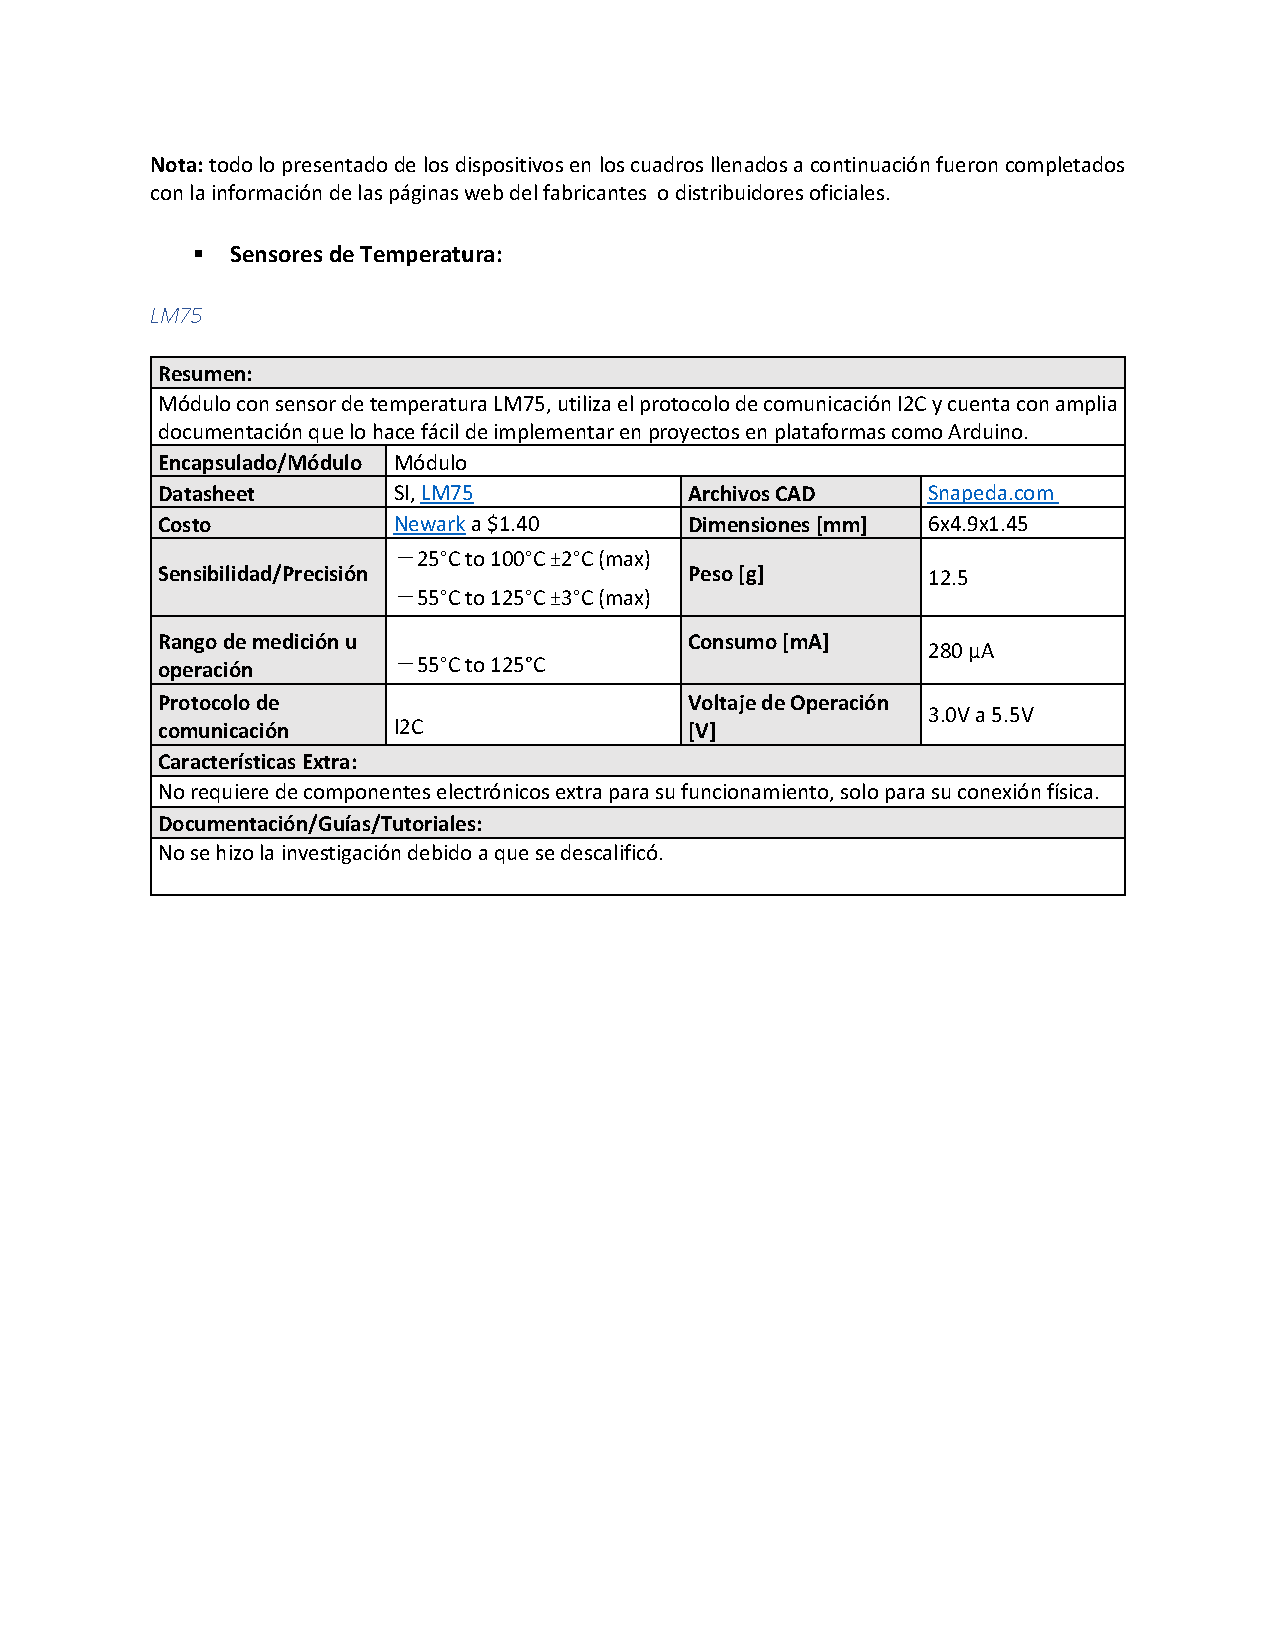
\includepdf[pages=-, scale=1]{document/annexes/seleccion_hardware.pdf}


\section{Diseño de Placa de Circuito para dimensionamiento de Subsistema de Navegación} \label{chp:anexo:pcb_layout_esquematico}

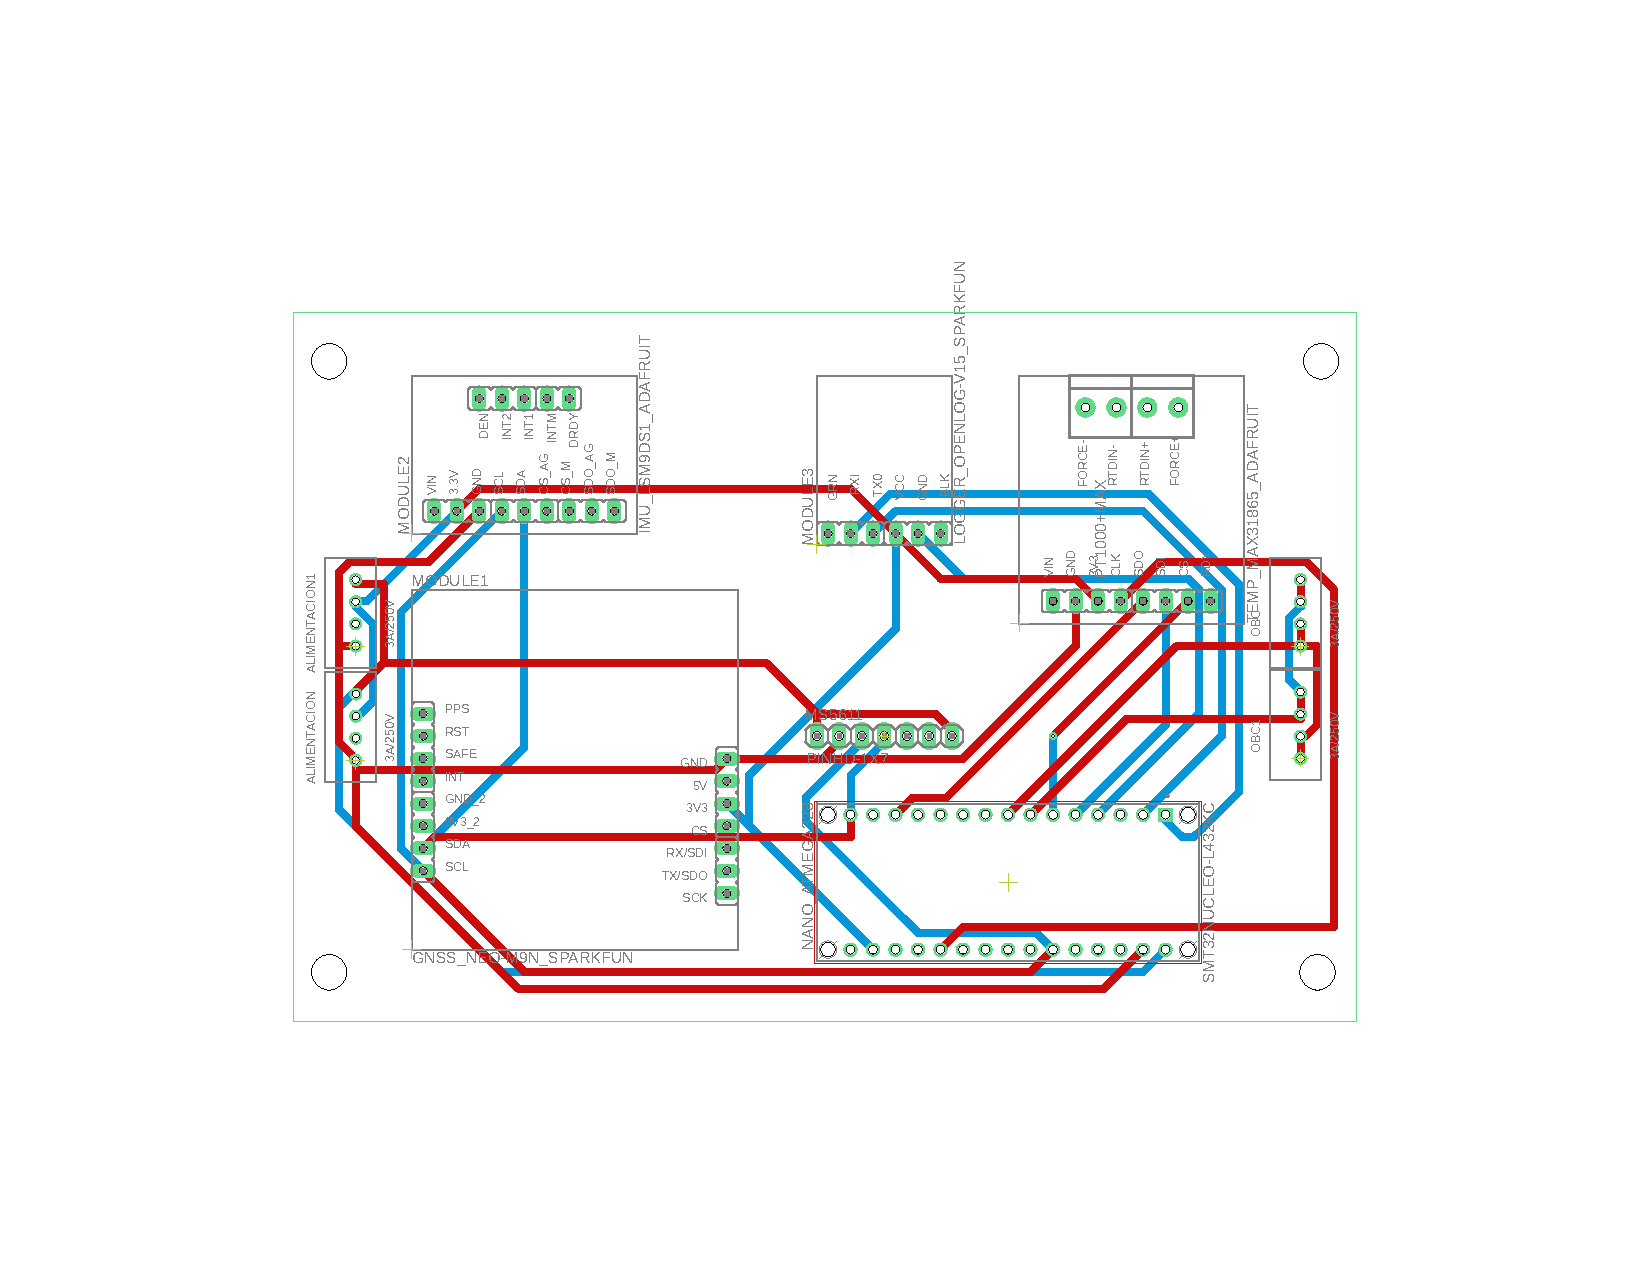
\includepdf[pages=-, angle=90]{document/annexes/PCB_layout.pdf}

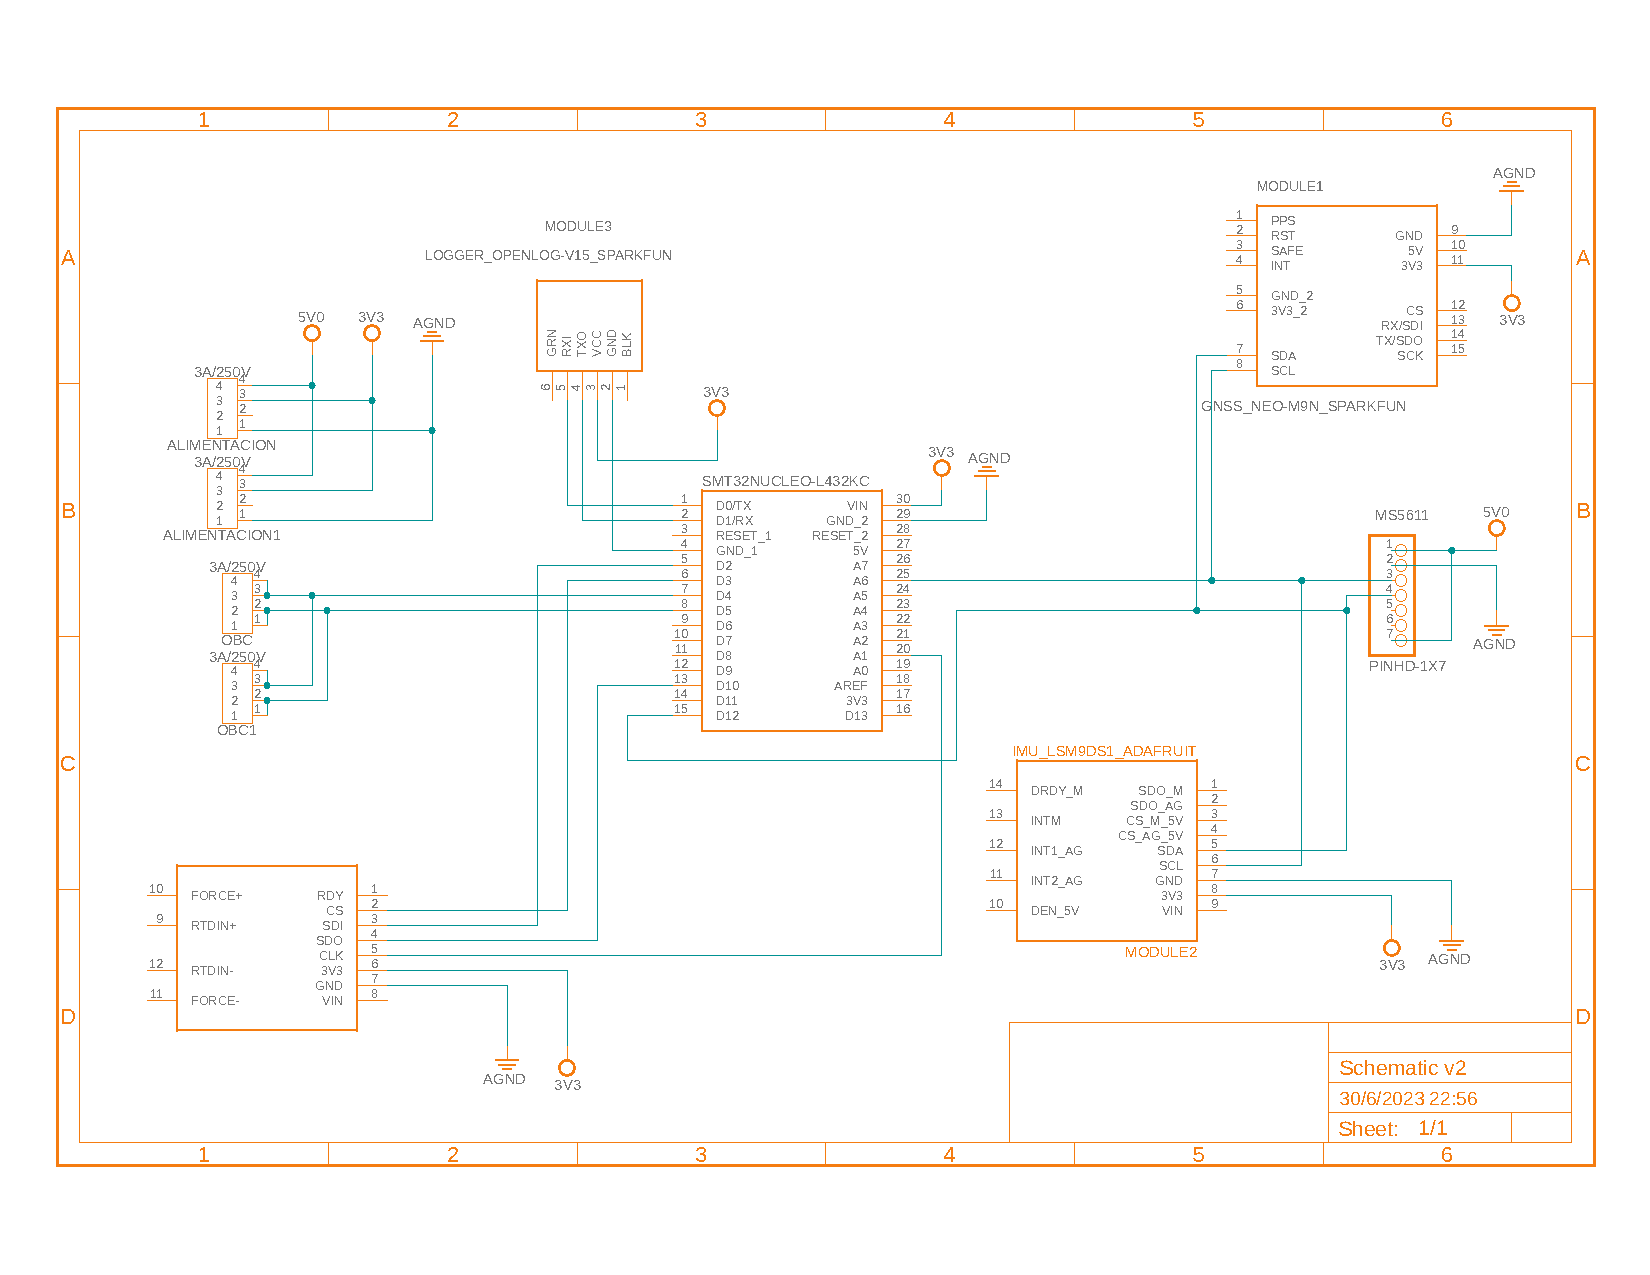
\includepdf[pages=-, angle=90, scale=0.8]{document/annexes/esquematico.pdf}

\newpage

\section{Recursos y herramientas}  \label{chp:anexo:source_thesis}

\begin{flushleft}
{\sffamily\small\textit{Las herramientas utilizadas fueron: }}

\begin{itemize}
    \item {\sffamily\bfseries\small\textit{\LaTeX     \space fue utilizado como editor de texto. Utilizando Overleaf.}}
    \item {\sffamily\bfseries\small\textit{Python junto con Jupyter Notebooks fue utilizado como herramienta de programación.  }}
\end{itemize}

\vspace{1cm}

{\sffamily\bfseries\small\textit{El código fuente y todo lo realizado en la presente fue cargado en un repositorio Online llamado GitHub, el repositorio online se puede visitar en el siguiente enlace: }}

\vspace{0.5cm}

\begin{center}
\href{https://github.com/osminlab/Proyec_Gda_Simula_PCB_Nav}{https://github.com/osminlab/Proyec\_Gda\_Simula\_PCB\_Nav}
\end{center} 

\vspace{0.5cm}

\textbf{Nota 1: } {\sffamily\small\textit{En el repositorio de GitHub se encuentran  muchos archivos README.md que guía y explican como está distribuido toda la información perteneciente a este trabajo de graduación.}}

\textbf{Nota 2:} {\sffamily\small\textit{Todas las imágenes son de autoría personal a menos que se diga lo contrario. Algunas imágenes son de búsqueda en Google con el filtro de 'Creative Commons licenses',  o de autores específicos que se han dado sus créditos respectivos en este trabajo. Además, se crea una carpeta llamada 'LICENSES' en el repositorio por todas las imágenes tomadas de tercero.}}
\end{flushleft}


